% E-meter software design, by Avery
\subsection{Software Design}

The typical programming paradigm for the MS430 is to
maximize the amount of time the processor spends in the sleep
state. To do this, many of the peripherals on the MS430 chip can be
configured to generate interrupts that wake the processor and execute
code relevant to the triggering events. The software designed for the
E-meter follows this paradigm of sleeping and interrupts, as pictured
in \ref{fig:emeter_software_flow}.

\begin{figure}[htbp]
\begin{center}
  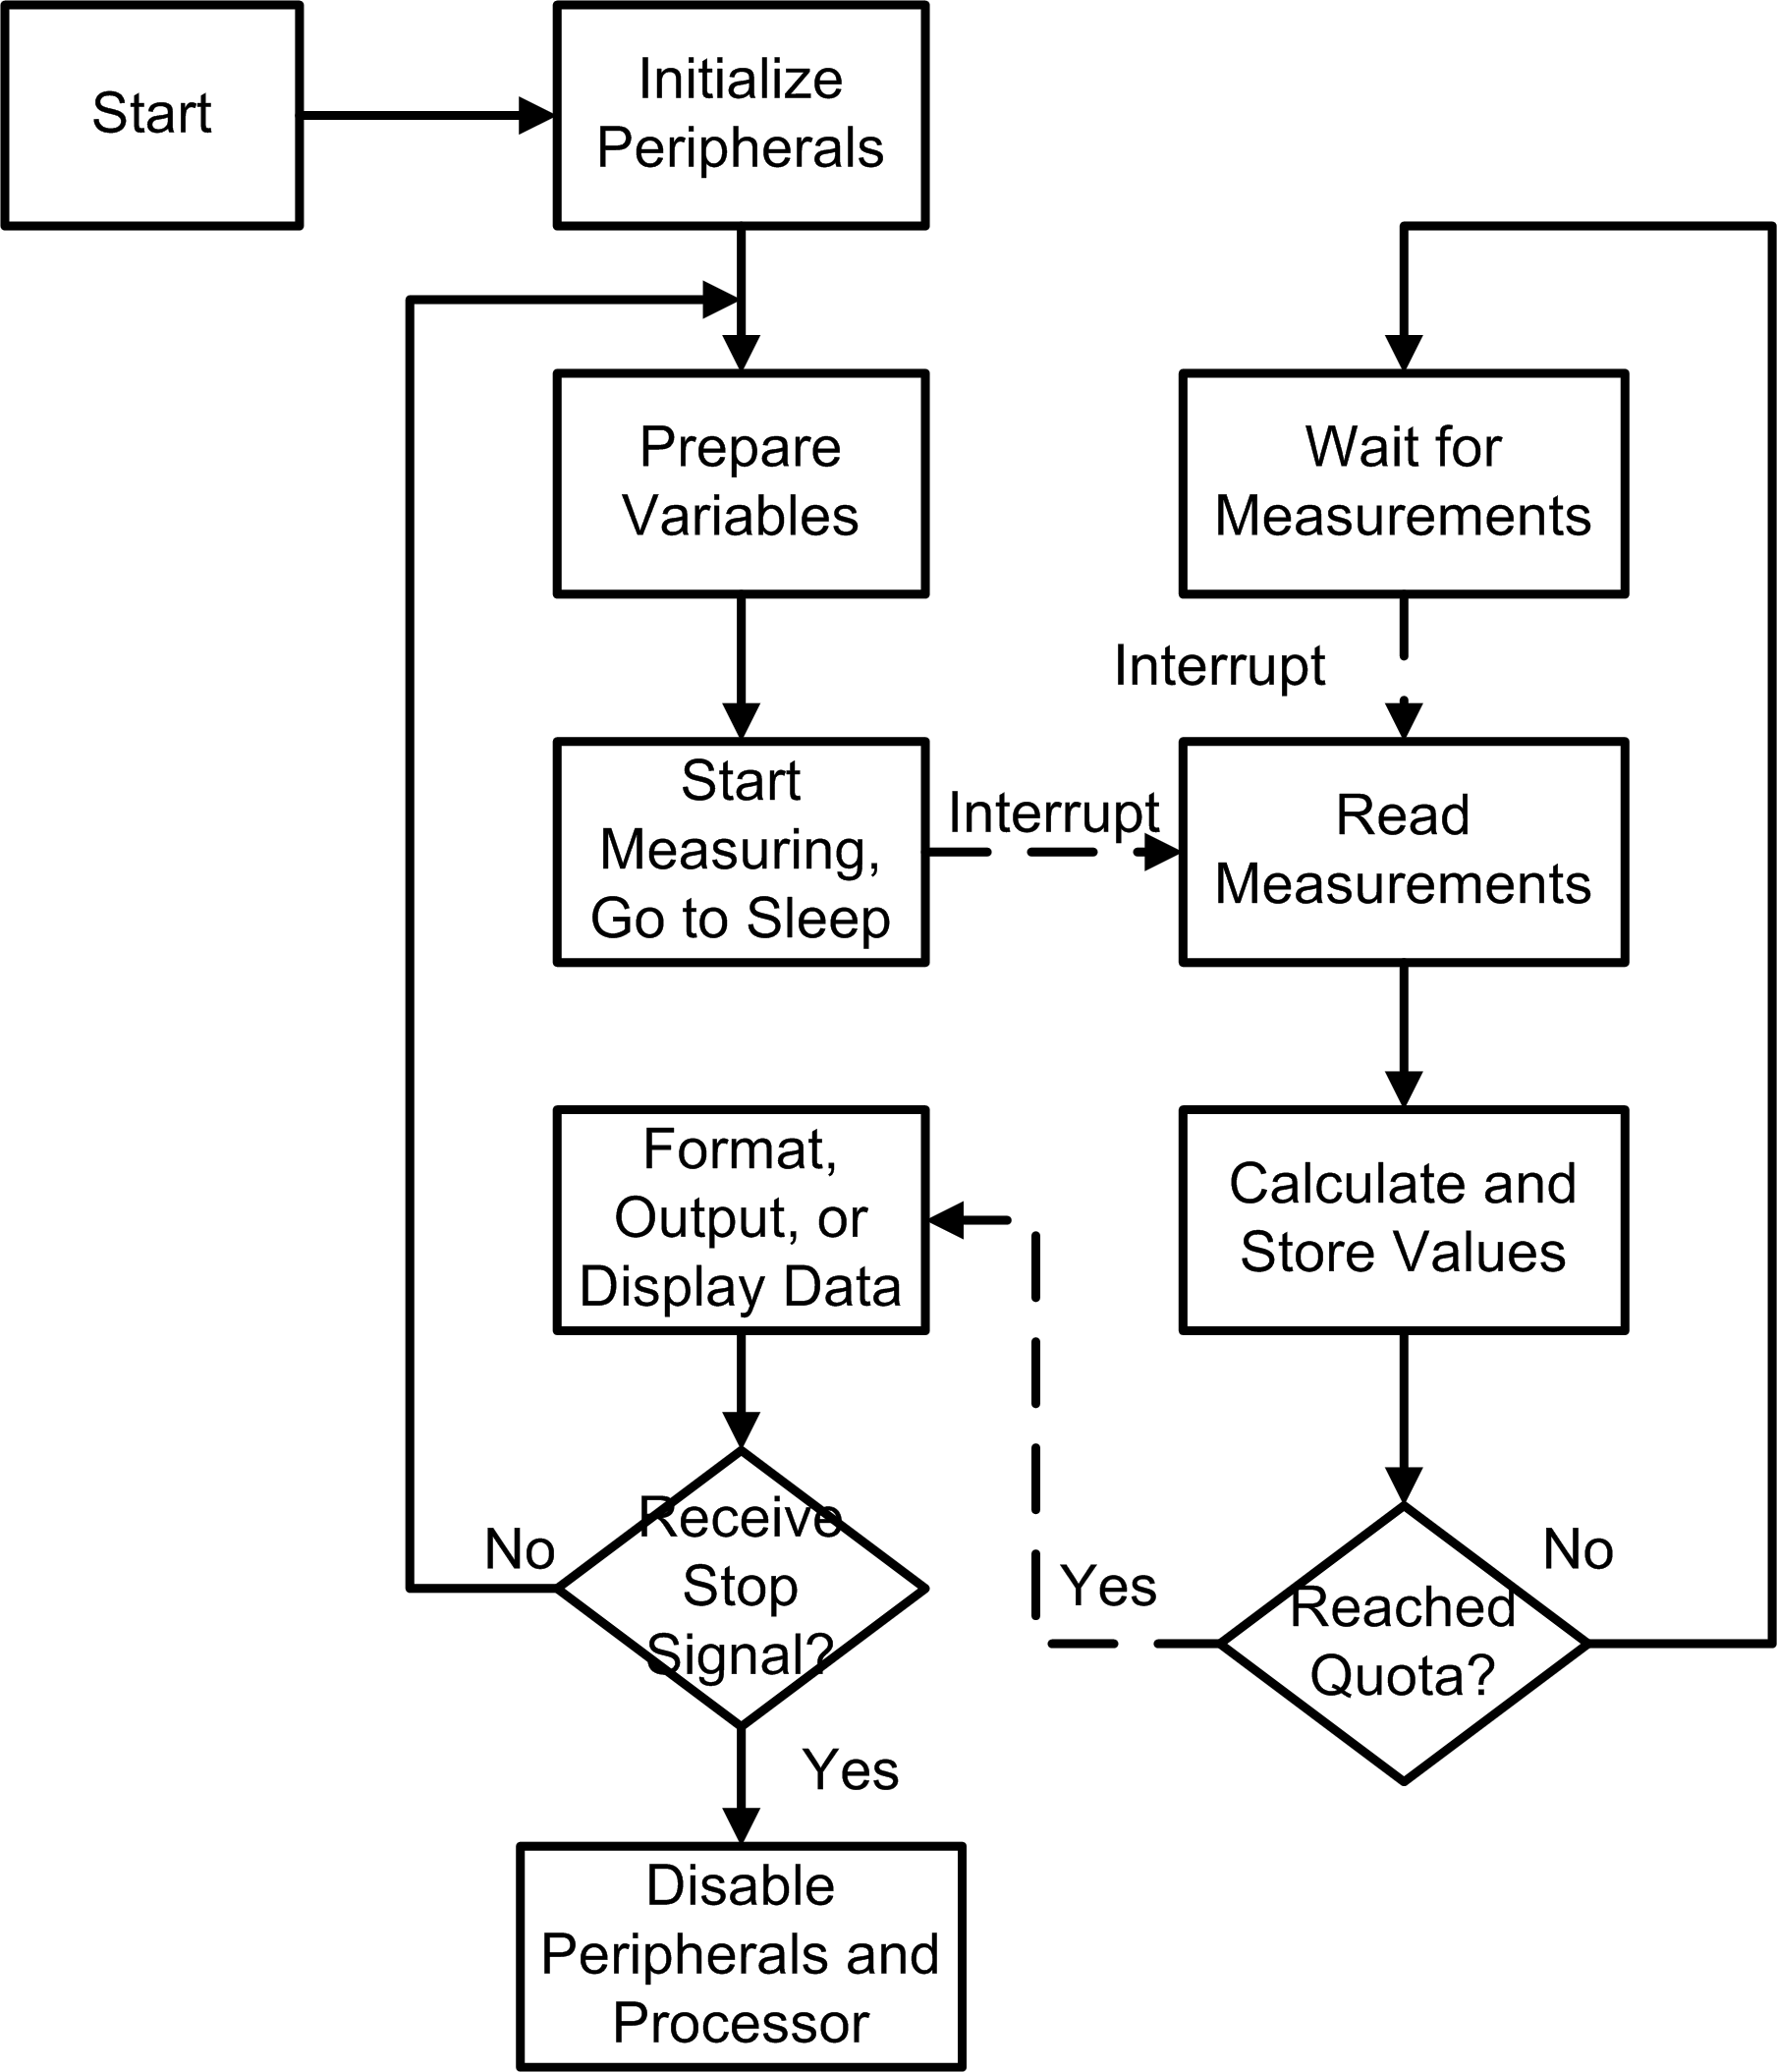
\includegraphics[width=5in]{includes/Emeter_Software_Flowchart}
  \caption{E-Meter Software Flow Diagram}
  \label{fig:emeter_software_flow}
\end{center}
\end{figure}

\subsubsection{Design}
The primary focus of the E-meter is measuring the current load and
line voltage of each phase of electricity entering the building. The
input networks for the E-meter convert these different elements into
voltages that the MSP430 can read on its dedicated \ac{ADC}
hardware. The E-meter software must allow time for these \acp{ADC} to
resolve the voltages, but must also output summaries of these
measurements to its built-in LCD screen and to the base station. To do
this, the software running in the E-meter first loads pre-defined
values into the device's configuration registers, then measures the
voltages on the \acp{ADC}, outputs a summary of the information
collected, then repeats the collection and output sections. For
simplicity, the conversion factors to map these values ranging from
$-0x8000$ to $0x7999$ into their real-world values (such as $\pm
120\sqrt{2}\volt$) are hard-coded into the program at compile time
using several \texttt{\#define} statements.

The initialization step loads values into the MSP430's configuration
registers that enable the desired features of the E-meter. The list of
possible values can be found in the MSP430 User Manual\cite{slau056j},
which design team referenced frequently in determining the values for a 
suitable configuration. In the current version of the software, the
first six \ac{ADC} channels are ``grouped'' together while the seventh is
disabled. Grouping the channels ensures that all six will measure at
the same time, and will only generate one interrupt that signals when
all six have finished measuring. The \acp{ADC} measure voltages
between $-0.6 \volt$ and $0.6 \volt$ and returns 16-bit
two's-complement integers that represent that range. The \ac{IEEE} 754
standard requires a 32-bit floating point number to have at least 23
binary places of precision, which could store several of these
readings without roundoff error. Additionally, the setup stage selects
the clocking frequency for the \acp{ADC} and for the serial \ac{UART},
selects which of the \acp{ADC} to measure, and which pins are used for
the \ac{LCD} display.

As the final task in this preparation stage, the program
enters a loop where the main calculations take place. At the beginning
of this loop, the processor enables the \acp{ADC} and puts the main
process to sleep.

When the \acp{ADC} have measured the voltage from their attached
circuits, the ``group leader'' may raises an interrupt to signal the
completion of the measurement. This interrupt triggers the \ac{ADC}
\ac{ISR}, which checks that the \ac{ISR} was indeed caused by one of
the active \acp{ADC}. After doing so, the \ac{ISR} turns off
the \acp{ADC}, preventing the \acp{ADC} from interrupting again before
the original interrupt can be cleared. the \ac{ISR} then reads the
volage and current for the first phase. It uses the hardware
multiplier to square the 16-bit-integer current and voltage
measurements into 32-bit square measurements, and also computes the
instantaneous power by multiplying the current by the voltage. Each of
these 32-bit integers are then summed with a corresponding 32-bit
floating-point number, a process which takes a considerable amount of
computation but allows for much larger numbers to be
represented. This is essential for computing RMS: in order to find the
mean of the squares, the squares must be summed together without
exceeding the limits on their representation. 32-bit \ac{IEEE} floating-point
numbers can express numbers up to $2^{127}$, which is many orders
greater than the $2^{31}$ limit on integers; hence, using
floating-point numbers for storing sums prevents overflow when a
limited number of sums are to be stored. The program defines a quota
for the number of samples to take before computing the mean and
outputting data. This limit means that a known number of items will be
summed, which not only prevents overflow but also ensures that the
output from the E-meter will occur at regular intervals. While a timer
could provide the desired regularity, connecting the output rate to
the measurement rate gives an implicit indication of the measurement
rate without requiring special debugging equipment.

In contrast with resetting the processor, waking the main process
resumes execution at the same location where it went to sleep. With
the newly-measured sum-of-squares for current and voltage for all
three channels, as well as the sum of instantaneous power during the
sampling period, the main process decides what it needs to calculate
for output. In the current version of the software, the E-meter
transmits power of all three phases and total power for each run
through the main loop; unless the \ac{LCD} screen displays current or
voltage, their \ac{RMS} values are unneeded. The main loop always
calculates power and energy consumed for output and accumulation,
respectively.

If necessary, the loop continues the computation of \ac{RMS} voltage
and current by first finding the mean of the squares by dividing the
sum of the squares by the number of measurements, then calculates the
square root of these mean squares, thereby giving the RMS measurement;
multiplying by the callibration factors gives the real-world voltage
or current. These values are then output to the LCD screen, as
detailed in the 

As the power is not measured by squaring, the power sum is simply
divided by the number of measurements to obtain the mean real power;
the energy total is incremented by the product of the power and the
time taken to perform the measurements and calculations, which one of
the timers tracks. By applying the callibrated conversion factors,
the software computes power in watts and the acculated power in
watt-hours. 

\subsubsection{User Interface}
In lieu of a working XBee network, the primary interface to the
E-meter uses the single touch-button and the \ac{LCD} screen. The LCD
display uses the four digit places in the upper-right corner to
display the current uptime in hours and minutes. The center dial
displays the seconds elapsed: every five seconds, another of its
twelve regions fills, until it resets at the end of each minute. The
upper-left characters indicate which of power, energy, current, or
voltage is displayed. The actual value is displayed in the six primary
characters.

The six primary characters show the real-time reading of the selected
value. The first character only indicates the sign of the number: it
is empty for positive values and shows a negative sign when the value
is negative. The next three characters display the value in one of two
forms: either a number from 10 to 999, or a decimal number less than
10 with two following decimal places. The software automatically
determines in which \ac{SI} range to place the value to fit these
forms. The fifth character displays this range: at the moment, this
will be one of ``k'', ``m'', or ``u'' for the prefixes kilo-, milli-,
and micro-, respectively; the space is blank if there is no
prefix. The final character shows the base unit of the measurement:
``A'' for current in amps, ``V'' for voltage in volts, ``W'' for power
in watts, and ``E'' for energy in watt-hours. As there is not enough
room for ``Wh'', ``E'' seemed the next most obvious character to put,
though it may cause confusion if users expect to see only \ac{SI}
units. At present, the power and energy measurements are totals from
all three phases, while the current and voltage read only from the
first phase.

The touch-button will turn on the \ac{LCD} backlight if it has gone to
sleep. If the backlight is on, the button will advance the display to
the next mode. This very simply interface has not been user-tested,
but its simplicity.

\subsubsection{Current Status}
The present software for the E-meter reads the current and voltage
from three separate inputs using six of the seven hardware \ac{ADC}
channels. These channels are grouped together, so they only trigger
the \ac{ISR} when all six have finished measuring. The

At present, the software collects readings from two of the MSP430's
\ac{ADC} ``channels'', simulating what an individual ``phase'' would
be measured. As mentioned in the MSP430 user's guide, these two
channels are grouped together, so they wait for each other to resolve
before triggering the \ac{ISR}. This approach can be extended to the
other channels; with only a few changes in software, all of the six
\acp{ADC} needed for this application can group together.

Laboratory execution and examination using a stopwatch show that the
current software can make approximately 760 measurements per second on
both channels when 120 measurements are taken to compute the \ac{RMS}
data before outputting over RS232.

%\subsubsection{Future Work}
%% We have the LCD and buttons working now